\begin{appendix}
\section{Kalibrierungen}
\subsection{Wei�lichtpunkt}
\label{subsec:weisslicht}
Fit (Abbildung \ref{fig:weisslichtpunkt_eichung_1}) und Parameter (Tabelle \ref{tab:weisslichtpunkt_eichung_1}) f�r die Kalibrierung des ersten Wei�lichtpunktes.

\begin{figure}[H]
\centering
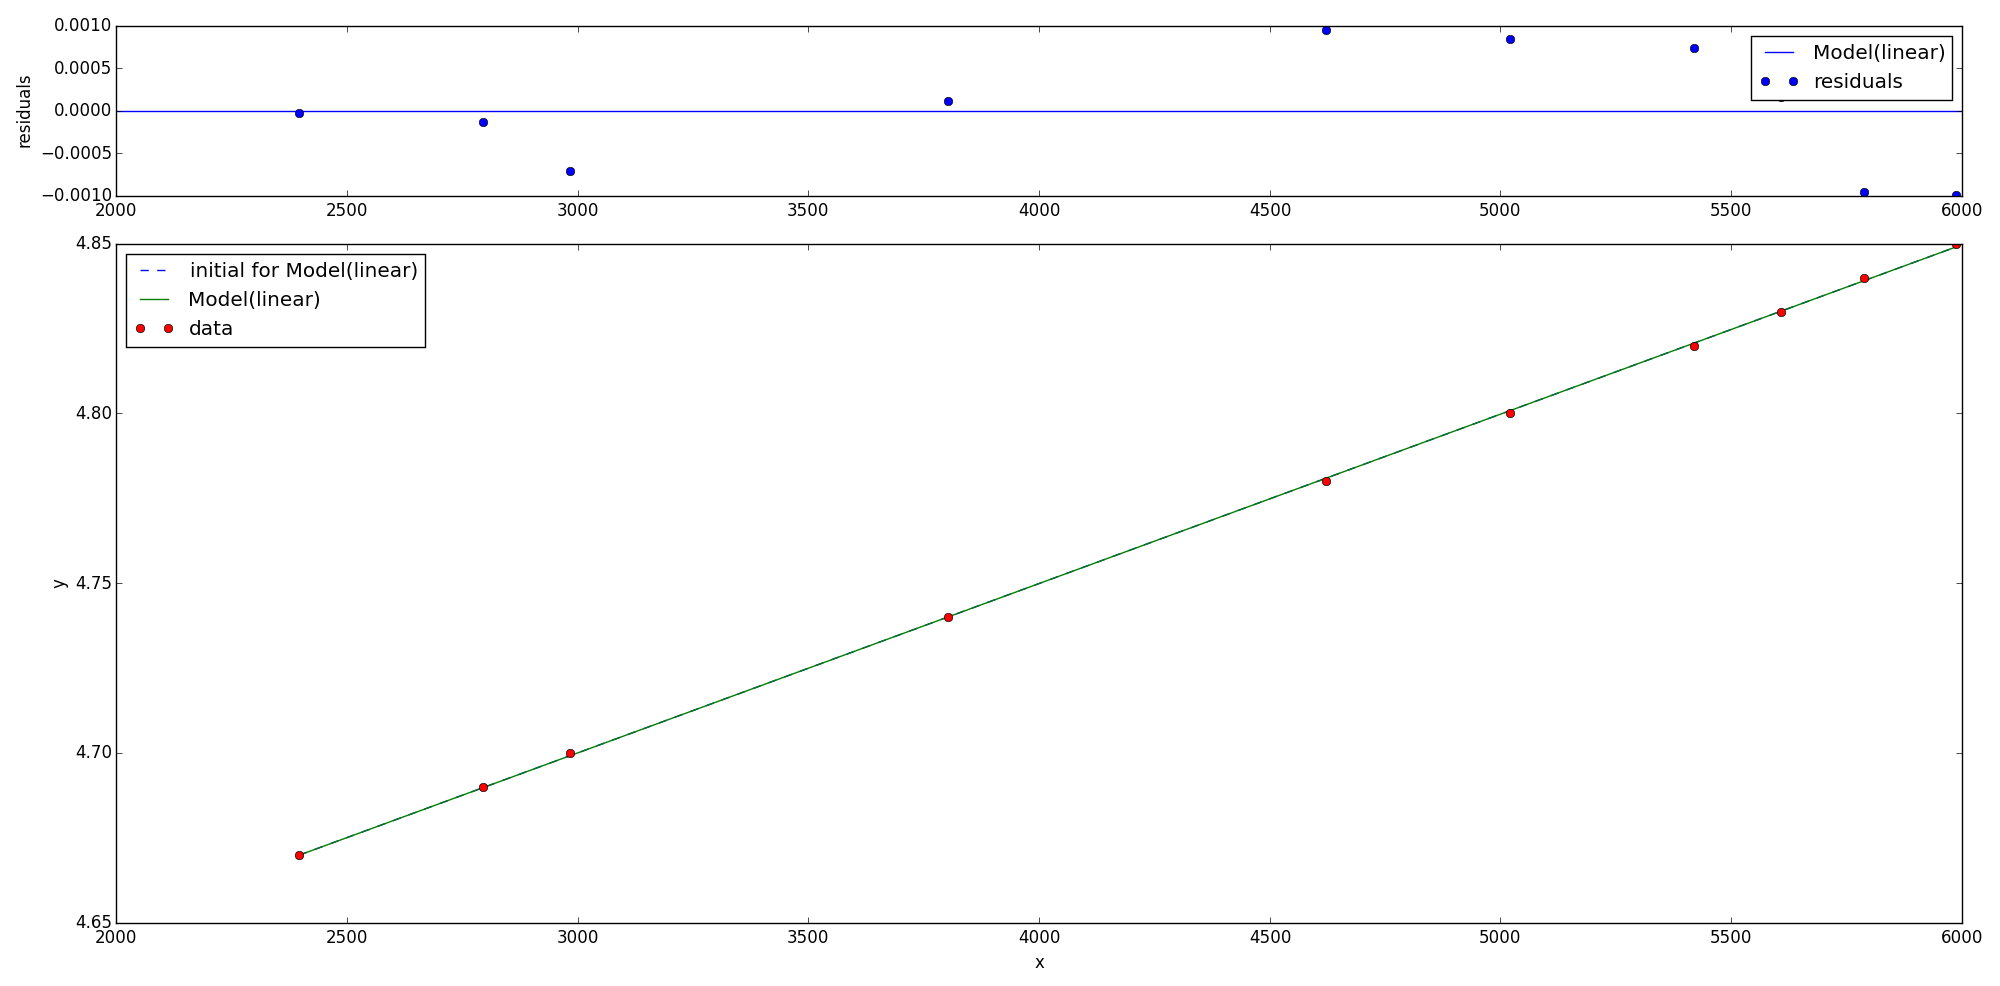
\includegraphics[scale = 0.33]{eichung_weisslicht_4,75.png}
\caption{Erster bestimmter Wei�lichtpunkt bei 4,755(8) mm}
\label{fig:weisslichtpunkt_eichung_1}
\end{figure}

\begin{table}[H]
\centering
\caption{Parameter des Fits f�r den ersten Wei�lichtpunkt}
\label{tab:weisslichtpunkt_eichung_1}
\begin{tabular}{|c|c|}
\hline Parameter & Wert \\ 
\hline A & 4.99(2)e-05 \\ 
\hline B & 4.5505(9) \\ 
\hline 
\end{tabular} 
\end{table}

Fit (Abbildung \ref{fig:weisslichtpunkt_eichung_2}) und Parameter (Tabelle \ref{tab:weisslichtpunkt_eichung_2}) f�r die Kalibrierung des zweiten Wei�lichtpunktes.

\begin{figure}[H]
\centering
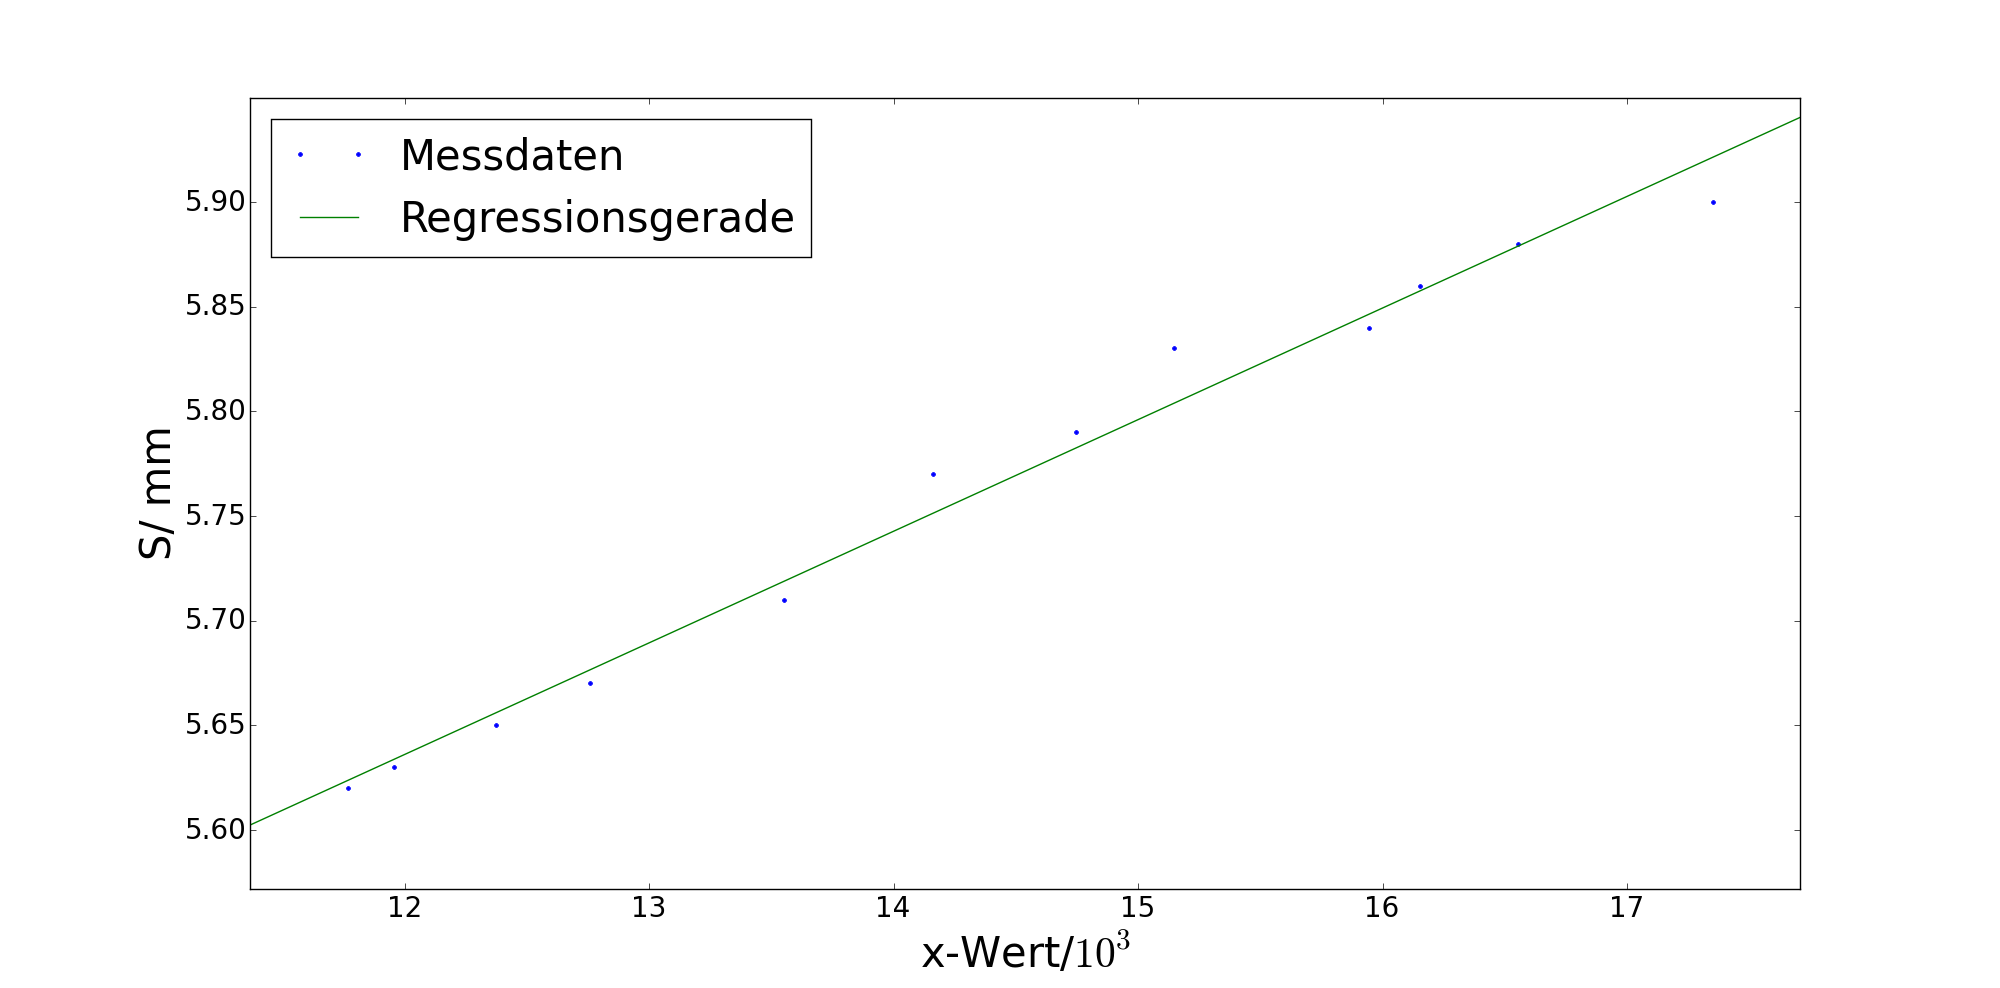
\includegraphics[scale = 0.33]{eichung_weisslicht_5,77.png}
\caption{Zweiter bestimmter Wei�lichtpunkt bei 5,770(3) mm}
\label{fig:weisslichtpunkt_eichung_2}
\end{figure}

\begin{table}[H]
\centering
\caption{Parameter des Fits f�r den zweiten Wei�lichtpunkt}
\label{tab:weisslichtpunkt_eichung_2}
\begin{tabular}{|c|c|}
\hline Parameter & Wert \\ 
\hline A & 5.3(2)e-05 \\ 
\hline B & 5.00(3) \\ 
\hline 
\end{tabular} 
\end{table}
\subsection{Wei�lichtpunkt mit Schmalbandfilter}
Fit f�r die Kalibrierung des ersten Wei�lichtpunktes mit Schmalbandfilter.
\begin{figure}[H]
\centering
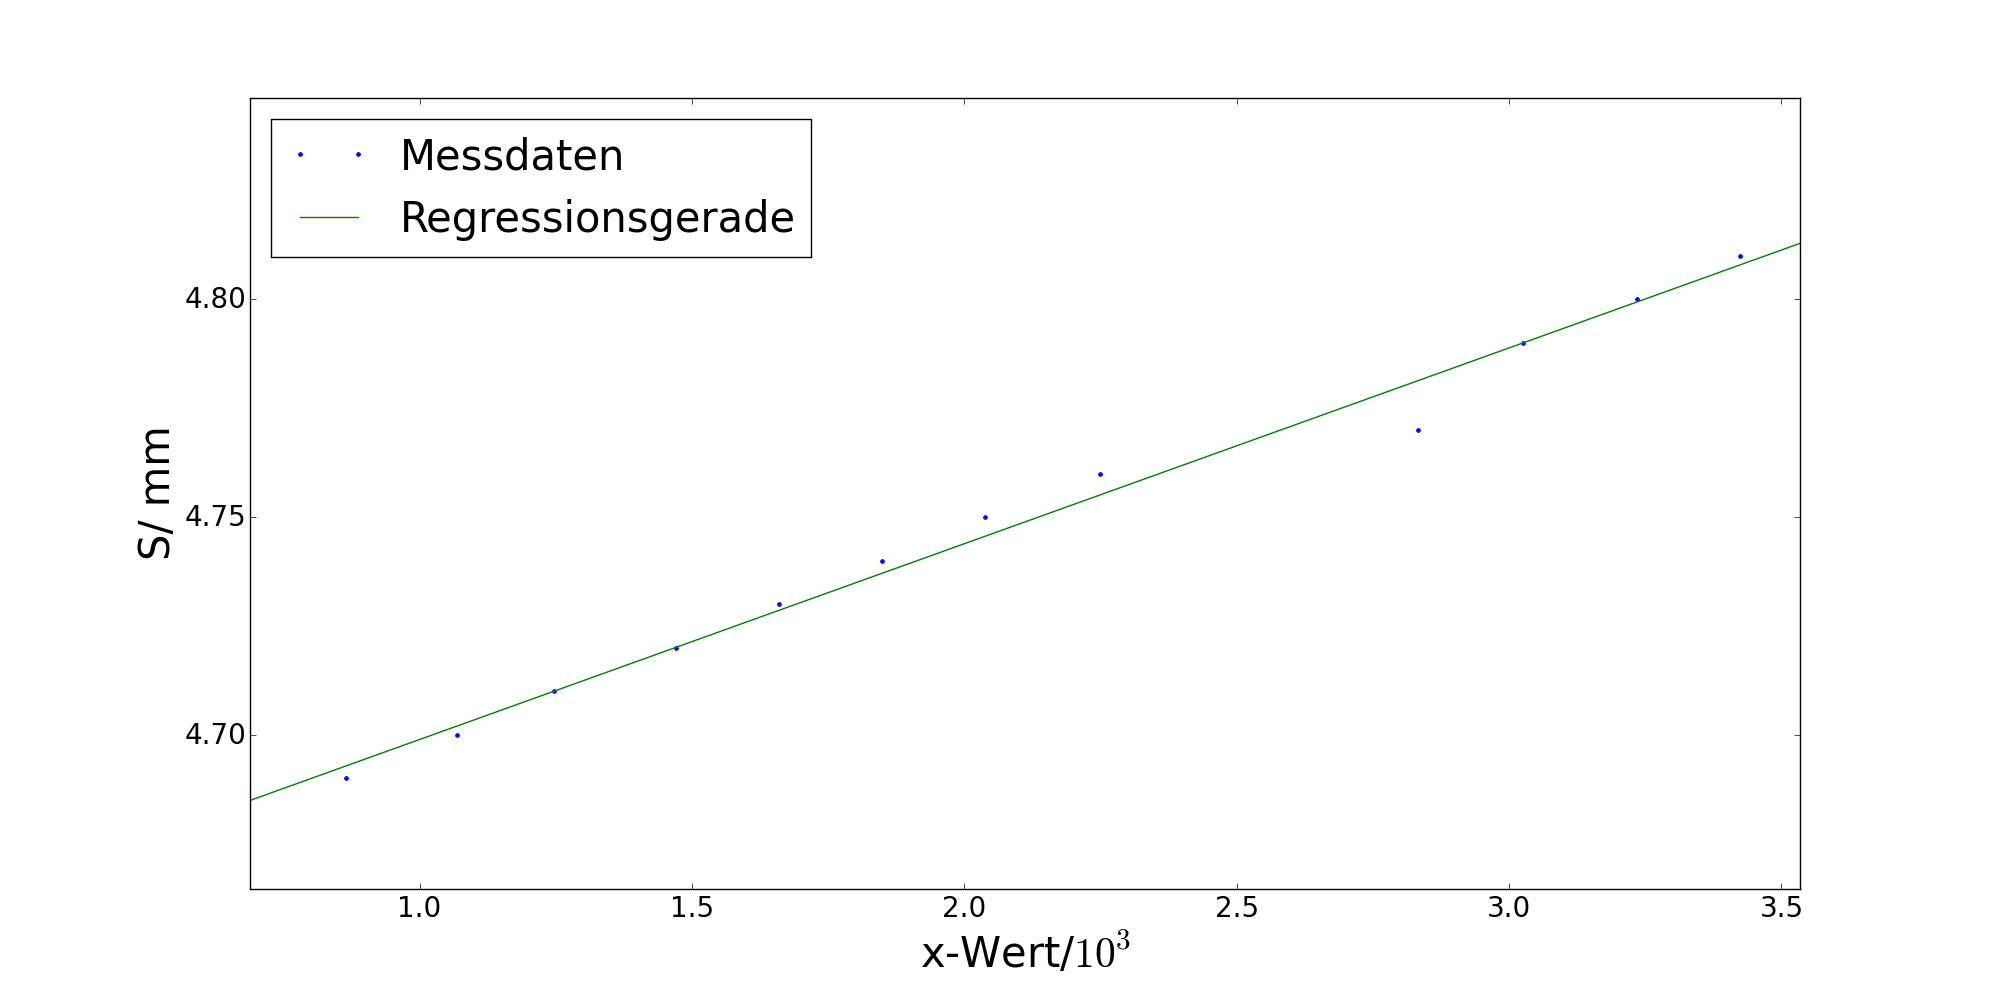
\includegraphics[scale = 0.33]{eichung_weisslicht_filter_4,75.png}
\caption{Erster bestimmter Wei�lichtpunkt bei \SI{4,755(8)}{mm} mit Schmalbandfilter}
\label{fig:weisslichtpunkt_eichung_filter}
\end{figure}

\begin{table}[H]
\centering
\caption{Parameter des Fits f�r die Kalibrierung mit Filter ($S(x) = Ax+B$)}
\label{tab:weisslichtpunkt_eichung_filter}
\begin{tabular}{|c|c|}
\hline Parameter & Wert \\ 
\hline A & 4.49(5)e-05 \\ 
\hline B & 4.654(3) \\ 
\hline 
\end{tabular} 
\end{table}
\subsection{Schwebung}
\label{Schwebung}
\begin{figure}[H]
\centering
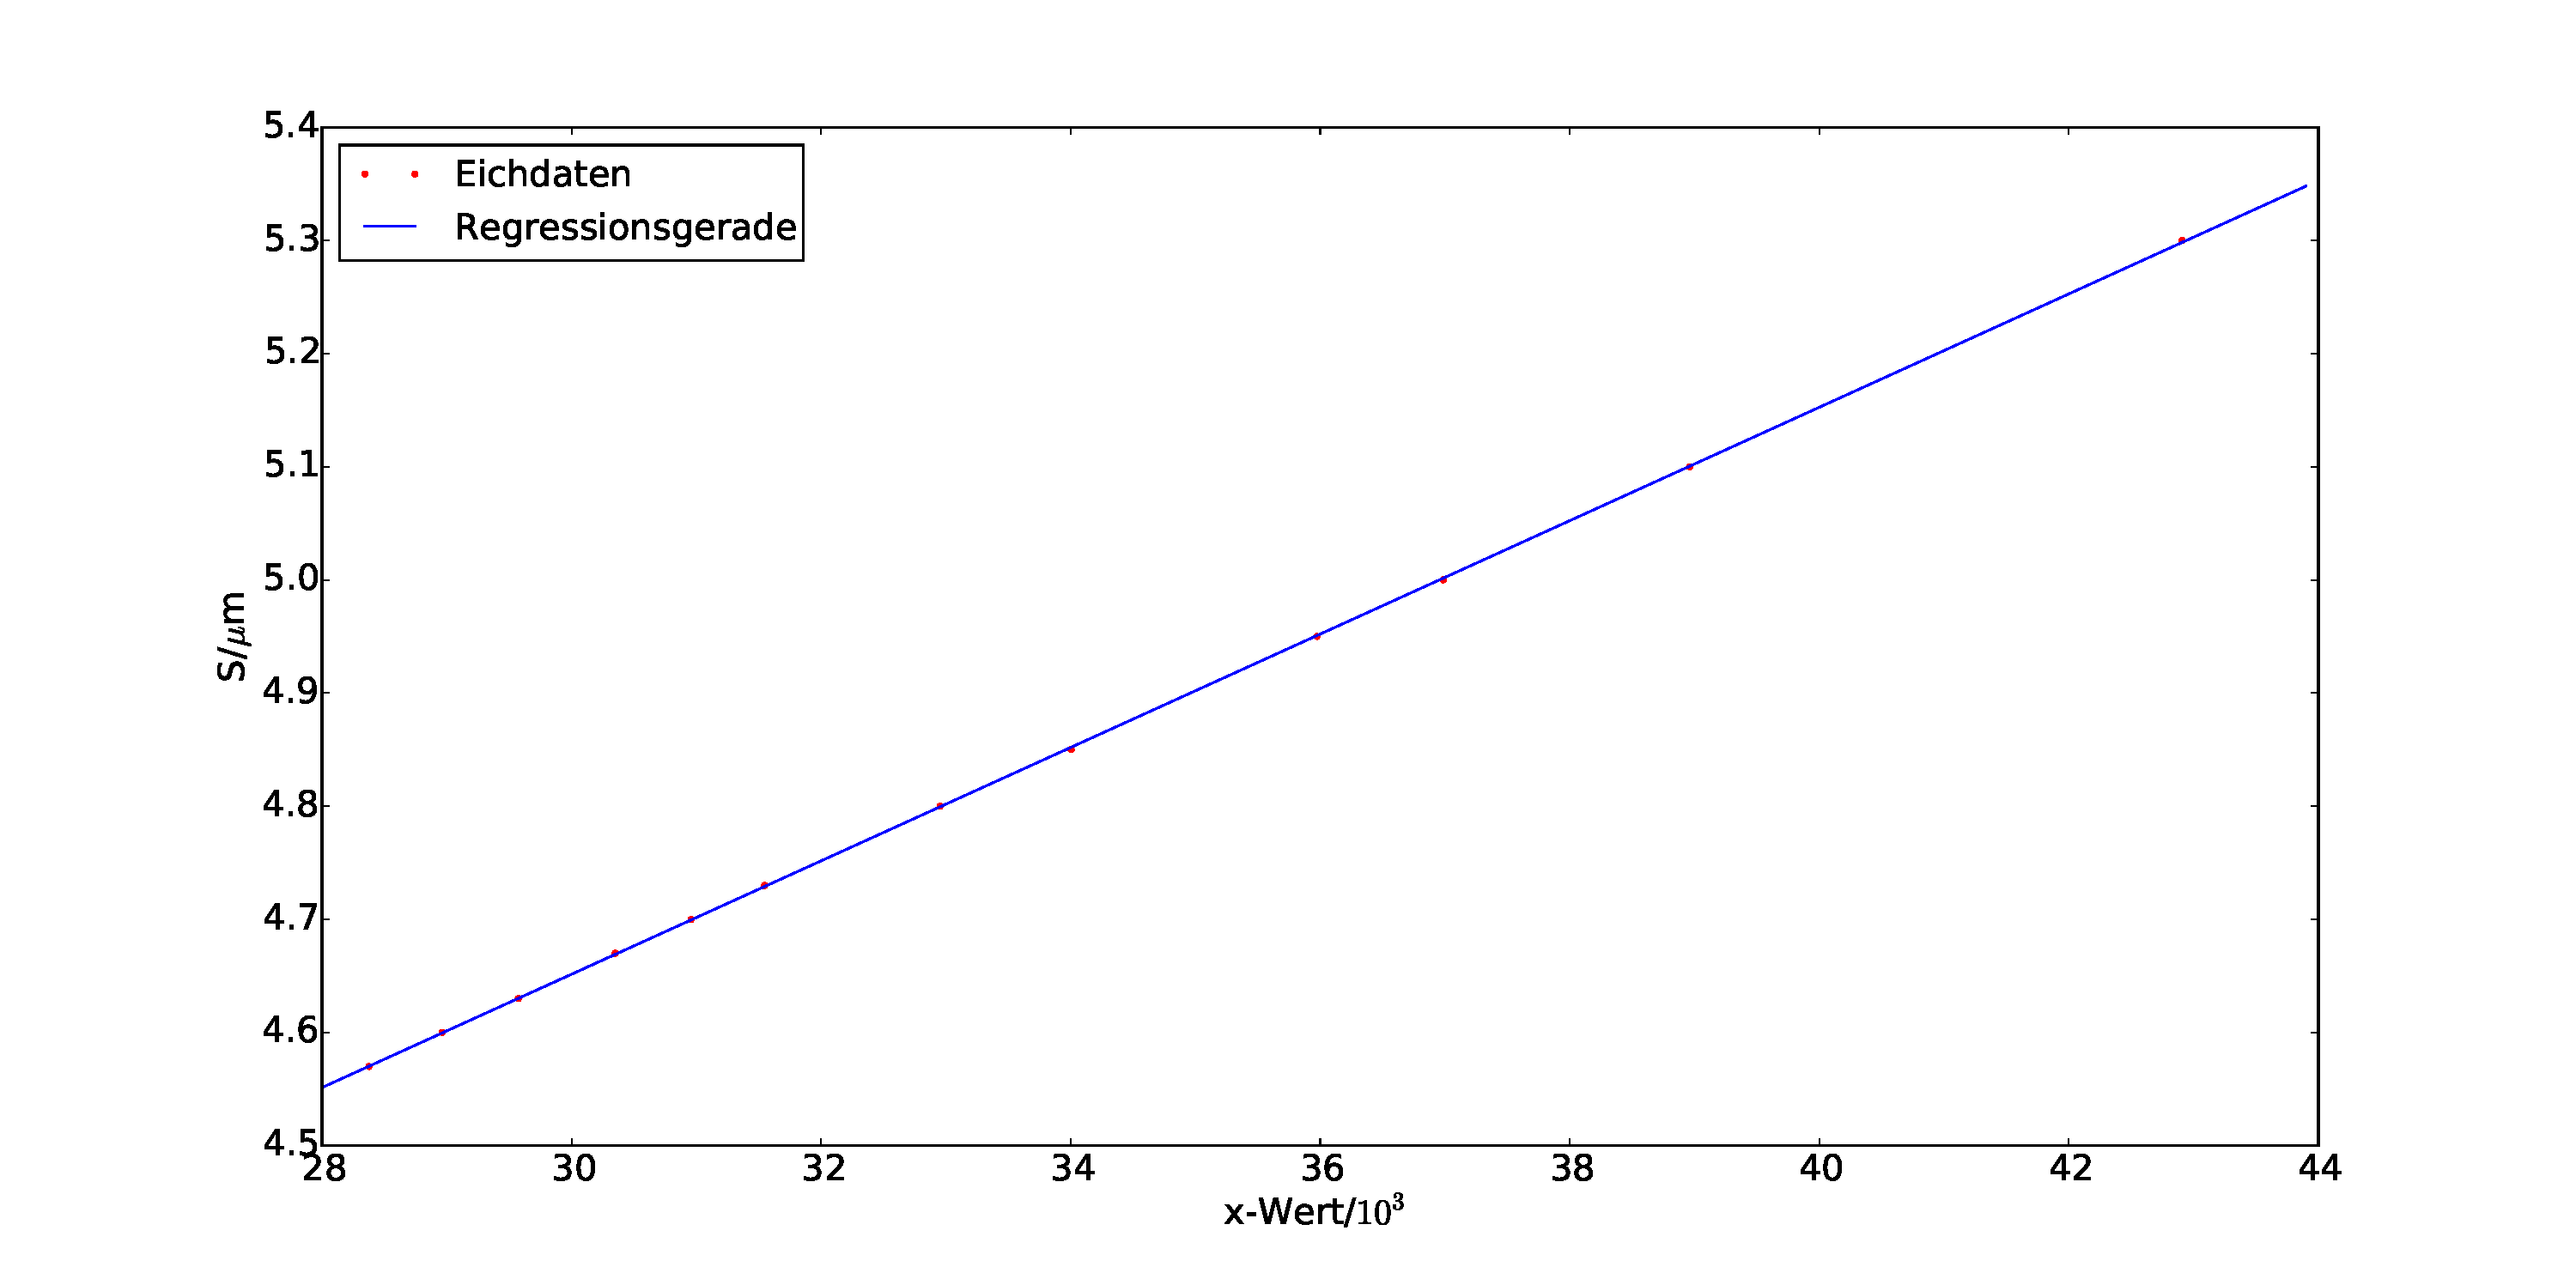
\includegraphics[scale = 0.28]{Eichdaten_Schwebung}
\caption{Kalibrierung f�r die Schwebung mit einer Fitfunktion $S(x)/\mu m= 5,010(8)\cdot10^{-5}\cdot x + 3.148(3)$. F�r die Berechnung des Fits wurde der Ursprung in den Schwerpunkt der Daten gelegt, um f�r den Fit unkorrelierte Fitparameter zu erhalten.}
\label{fig:Schwebung_Kalibrierung}
\end{figure}

\end{appendix}